% !TeX program = xelatex
\documentclass[9pt]{ctexbeamer}
\usepackage{style/shubeamer}
\usepackage{amsmath,amssymb,booktabs,graphicx,hyperref,tikz}
\setmainfont{CMU Serif}
\setsansfont{CMU Sans Serif}
\graphicspath{{figures/}}
% Generated by the executed Chapter 11 notebook.
\newcommand{\SampleYear}{2025}
\newcommand{\SourceRows}{6,888,585}
\newcommand{\SourceCodes}{5830}
\newcommand{\SampleRows}{1,313,872}
\newcommand{\SampleCodes}{5,500}
\newcommand{\SampleDays}{243}
\newcommand{\SnapshotCodes}{5,458}
\newcommand{\SampleEnd}{2025-12-31}
\newcommand{\ReturnMean}{0.168}
\newcommand{\ReturnMedian}{0.000}
\newcommand{\ReturnStd}{4.214}
\newcommand{\ReturnLow}{-7.974}
\newcommand{\ReturnHigh}{10.009}
\newcommand{\ReturnMin}{-89.33}
\newcommand{\ReturnMax}{1211.11}
\newcommand{\ReturnSkew}{60.48}
\newcommand{\ReturnKurt}{10536.94}
\newcommand{\TargetCum}{2.63}
\newcommand{\TargetVol}{16.01}
\newcommand{\TargetMdd}{-13.96}
\newcommand{\TargetCount}{243}
\title[股票日频收益率分析]{Python金融数据分析}
\subtitle{第11章\quad 股票日频收益率分析}
\author[王伟冠]{王伟冠\quad 经济学院金融系}
\institute[SHU]{上海大学}
\date{\today}
\newcommand{\nbref}[1]{\par\vspace{0.12cm}{\scriptsize\color{shugray}对应 Notebook：#1}}
\newcommand{\sourcehint}[2]{\par{\tiny\color{shugray}\href{#1}{来源：#2}}}
\begin{document}
\begin{frame}\titlepage\end{frame}

\begin{frame}{本章从一张股票日表开始}
  \begin{block}{三个问题}
    一只股票今天涨了多少？\quad 一段时间持有的回报是多少？\par
    不同股票的收益分布与波动程度有什么差别？
  \end{block}
  \begin{enumerate}
    \item 了解中国 A 股市场的交易所、板块与证券代码。
    \item 读懂股票日数据中的价格、回报率、成交量与市值。
    \item 用 pandas 制作累计收益率、波动率、回撤和换手率。
    \item 用描述性统计与图表解释样本，并检查结果是否合理。
  \end{enumerate}
\end{frame}

\begin{frame}{本章路线}
  \tableofcontents
\end{frame}

\section{A股市场与股票日数据}
\begin{frame}{中国 A 股市场：交易所与板块}
  A 股是人民币普通股票。交易所是交易组织层级，板块是其市场分层。
  \vspace{0.4cm}
  \begin{columns}[T,totalwidth=\textwidth]
    \begin{column}{0.31\textwidth}
      \begin{block}{上海证券交易所}
        \textbf{主板}\par 成熟企业的重要上市市场\vspace{0.2cm}\par
        \textbf{科创板}\par 面向科技创新企业
      \end{block}
    \end{column}
    \begin{column}{0.31\textwidth}
      \begin{block}{深圳证券交易所}
        \textbf{主板}\par 含原中小板\vspace{0.2cm}\par
        \textbf{创业板}\par 服务创新创业企业
      \end{block}
    \end{column}
    \begin{column}{0.31\textwidth}
      \begin{block}{北京证券交易所}
        服务\textbf{创新型中小企业}\par
        2021年11月15日开市交易
      \end{block}
    \end{column}
  \end{columns}
  \vspace{0.25cm}
  深市主板与中小板于 \textbf{2021年4月6日}合并；本章不再把中小板作为独立现行板块。
  \sourcehint{https://star.sse.com.cn/assortment/stock/list/share/}{上交所股票分类}
  \sourcehint{https://www.szse.cn/aboutus/trends/news/t20210406_585442.html}{深交所两板合并公告}
  \sourcehint{https://www.bse.cn/company/introduce.html}{北交所简介；官网核对日期2026-09-09}
\end{frame}

\begin{frame}{用数据字段识别市场}
  \centering
  \begin{tabular}{cll}
    \toprule
    \texttt{Markettype} & 字段说明中的类别 & 本章处理 \\
    \midrule
    1 & 上证A股，不含科创板 & 沪市主板 \\[4pt]
    4 & 深证A股，不含创业板 & 深市主板 \\[4pt]
    16 & 创业板 & 保留 \\[4pt]
    32 & 科创板 & 保留 \\[4pt]
    64 & 北证A股 & 保留 \\[4pt]
    2 / 8 & 沪市B股 / 深市B股 & 本章排除 \\
    \bottomrule
  \end{tabular}
  \begin{itemize}
    \item \texttt{Stkcd} 保存为六位字符串：\texttt{000001} 不能读成整数 1。
    \item 市场类别、公司行业、ST 状态是不同维度。
    \item 本包没有证券简称、行业和代码变更映射；不能仅据代码判断跨期公司身份。
  \end{itemize}
  \nbref{第1节；映射依据包内字段说明}
\end{frame}

\begin{frame}{一行代表什么？股票代码 $\times$ 日期}
  \begin{block}{面板数据的两个维度}
    同一只股票在不同日期的记录构成\textbf{时间序列}；\par
    同一天不同股票的记录构成\textbf{横截面}。
  \end{block}
  \begin{center}
    \begin{tabular}{llrr}
      \toprule
      股票代码 & 日期 & 收盘价 & 日回报率 \\
      \midrule
      000001 & 2021-08-16 & 19.950 & 0.003017 \\
      000001 & 2021-08-17 & 19.670 & -0.014035 \\
      000001 & 2021-08-18 & 20.620 & 0.048297 \\
      \bottomrule
    \end{tabular}
  \end{center}
  \begin{itemize}
    \item 行的候选主键是 \texttt{Stkcd + Trddt}，不能只按日期去重。
    \item 日频数据汇总一天的交易，不能还原盘中的价格路径。
    \item 收益率以小数存储：\texttt{0.01} 表示 \textbf{1\%}。
  \end{itemize}
  \nbref{第2节；表中为原始包首三条记录}
\end{frame}

\begin{frame}{原始数据包：先核对覆盖范围}
  \begin{center}
    \begin{tabular}{ll}
      \toprule
      来源 & 本地 CSMAR 授权数据包 \\
      CSV 文件数 & 7 \\
      总记录数 & \SourceRows \\
      证券代码数 & \SourceCodes{}（包含A股、B股）\\
      字段数 & 27 \\
      日期范围 & 2021-08-16 至 2026-08-13 \\
      教学年份代码与日期重复键 & 0 \\
      \bottomrule
    \end{tabular}
  \end{center}
  数据限已有授权范围使用；代码数是本包中出现的代码数，不能直接当作官方历史上市公司总数。
  \nbref{2.1–2.5：从原始ZIP读取并计算概况}
\end{frame}


\begin{frame}[fragile]{第一步：查看压缩包，再执行解压}
\begin{lstlisting}[numbers=none]
import zipfile
with zipfile.ZipFile(zip_path) as archive:
    print(archive.namelist())
    for member in archive.infolist():
        target = (RAW_DIR / member.filename).resolve()
        assert target.is_relative_to(RAW_DIR.resolve())
        if not target.exists():
            archive.extract(member, RAW_DIR)
\end{lstlisting}
  \begin{itemize}
    \item Notebook从\texttt{data/}中的原始ZIP开始，解压到\texttt{data/raw/}。
    \item 先查看清单：7个CSV，以及字段说明和版权说明。
    \item 重复运行时保留已有文件；Windows与macOS使用相同的Python代码。
  \end{itemize}
  \nbref{2.1–2.2；路径变量在第2节设置，调用与输出都在Notebook中}
\end{frame}

\begin{frame}[fragile]{第二步：先试读，弄清列名与类型}
\begin{lstlisting}[numbers=none]
preview = pd.read_csv(
    csv_paths[0], nrows=5, encoding="utf-8-sig",
    dtype={"Stkcd": "string"},
    parse_dates=["Trddt", "Capchgdt"]
)
display(preview)
display(preview.dtypes)
\end{lstlisting}
  \begin{itemize}
    \item \texttt{nrows=5}：先看5行，确认原文件结构。
    \item 字符串代码保留开头的零；日期类型支持提取年份。
    \item 同时打开刚解压的TXT字段说明，确认收益率与金额单位。
  \end{itemize}
  \nbref{2.3；CSV是文本，读入后才成为pandas的DataFrame}
\end{frame}

\begin{frame}[fragile]{第三步：逐块读取，合并教学年份}
\begin{lstlisting}[numbers=none]
year_parts = []
for csv_path in csv_paths:
    reader = pd.read_csv(
        csv_path, dtype={"Stkcd": "string"},
        parse_dates=["Trddt", "Capchgdt"],
        chunksize=150_000, encoding="utf-8-sig")
    for chunk in reader:
        year_parts.append(
            chunk.loc[chunk["Trddt"].dt.year.eq(YEAR)].copy())
raw = pd.concat(year_parts, ignore_index=True)
\end{lstlisting}
  每次读取15万行，仅保留教学年份；\texttt{concat}将各块按行拼接。\par
  Notebook同时统计各文件行数和全包覆盖，再检查年度重复键与价格关系。
  \nbref{2.4–2.5；这里展示读取主线，完整计数与检查见Notebook}
\end{frame}

\section{筛选样本与检查口径}
\begin{frame}{先读懂三个标识，再开始统计}
  \begin{description}
    \item[市场类型] \texttt{Markettype} 用于筛选 A 股与区分板块。
    \item[填充标识] \texttt{Filling=0} 为正常原始交易记录；1、2 分别表示非节假日和节假日填充。
    \item[交易状态] \texttt{Trdsta=1} 为正常状态；2 为 ST，3 为 *ST，另有历史状态代码。
  \end{description}
  \begin{block}{填充记录不等于新增交易观测}
    如果直接统计全部记录，补入的零收益可能改变均值、波动率和零收益占比。
  \end{block}
  \begin{itemize}
    \item 主样本保留 ST 与极值，但剔除填充记录。
    \item 同时比较只保留正常状态的子样本，展示口径敏感性。
    \item 未缺失不等于没有质量问题；需要检查经济含义和字段之间的关系。
  \end{itemize}
  \nbref{2.6、3.1}
\end{frame}

\begin{frame}[fragile]{样本筛选}
\begin{lstlisting}[numbers=none]
a_share = raw[raw["Markettype"].isin([1,4,16,32,64])]
actual = a_share[a_share["Filling"].eq(0)]
traded = actual[
    actual["Dnshrtrd"].gt(0) & actual["Clsprc"].gt(0)
]
df = traded[
    np.isfinite(traded["Dretwd"]) & traded["Dretwd"].gt(-1)
].copy()
\end{lstlisting}
  \begin{center}
    \begin{tabular}{lr}
      \toprule
      2025年筛选步骤 & 记录数 \\
      \midrule
      原始记录（含B股、填充） & 1,435,881 \\
      A股记录 & 1,414,730 \\
      非填充且有成交、收益可用 & \SampleRows \\
      \bottomrule
    \end{tabular}
  \end{center}
  最终包含 \SampleCodes{} 个代码、\SampleDays{} 个样本日期。这里描述的是\textbf{有成交的股票日}。
  \nbref{第3节；原始记录保留在解压后的CSV中}
\end{frame}

\begin{frame}{数据检查：程序检查与业务判断配合}
  \begin{tabular}{p{0.38\textwidth}p{0.52\textwidth}}
    \toprule
    检查 & 本包结果与处理 \\
    \midrule
    股票代码 + 日期重复 & 教学年份未发现重复键，不自动去重 \\[7pt]
    非填充记录的价格、量 & 无非正收盘价、负成交股数、高低价顺序矛盾 \\[7pt]
    收益率边界 & 未发现含红利收益率小于等于 -100\% \\[7pt]
    缺失值 & 盘后成交、涨跌停字段等有缺失；不能一律填0 \\[7pt]
    特别大的涨跌幅 & 保留并查事件；不能统一截到正负10\% \\
    \bottomrule
  \end{tabular}
  \nbref{2.5、2.6、6节极值核验}
\end{frame}

\begin{frame}{样本板块构成：固定一个观察日期}
  \centering
  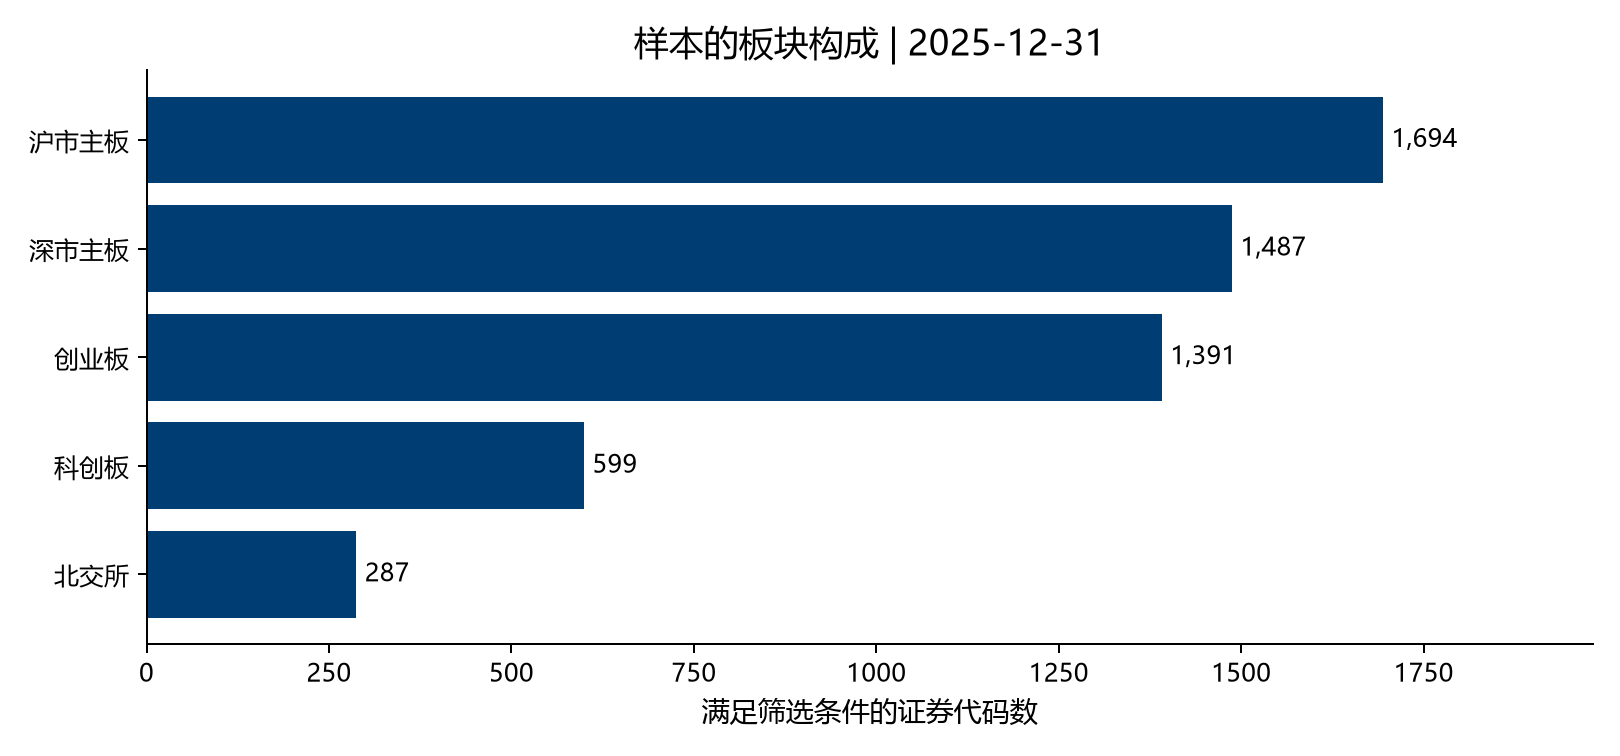
\includegraphics[width=.97\textwidth,height=5.25cm,keepaspectratio]{board_composition.png}
  \begin{itemize}
    \item \SampleEnd{} 当天有 \SnapshotCodes{} 个满足条件的证券代码。
    \item 分母是当日有成交、收益可用的样本；不等于交易所公布的上市公司数。
  \end{itemize}
  \nbref{3.2：\texttt{groupby + nunique}}
\end{frame}

\section{收益率与基础指标}
\begin{frame}{价格变化、交易所涨跌幅、含红利回报}
  \begin{tabular}{p{0.25\textwidth}p{0.32\textwidth}p{0.31\textwidth}}
    \toprule
    指标 & 计算或字段 & 关注点 \\
    \midrule
    未复权价格变化 & $P_t/P_{t-1}-1$ & 可能受分红、送转等影响 \\[8pt]
    交易所涨跌幅 & \texttt{ChangeRatio} & 使用可能已除权的交易所昨收价格 \\[8pt]
    不含现金红利回报 & \texttt{Dretnd} & 不考虑现金红利 \\[8pt]
    含红利回报 & \texttt{Dretwd} & 考虑现金红利再投资，本章主口径 \\
    \bottomrule
  \end{tabular}
  \begin{block}{价格跌了，持有回报就一定为负吗？}
    除息可能让价格下降，而持有者收到现金红利。需要先说明回报口径，不能只看价格曲线。
  \end{block}
  \nbref{第4节；以原包字段定义为准}
\end{frame}

\begin{frame}[fragile]{收益率计算：先排序，再找到正确的上期}
\begin{lstlisting}[numbers=none]
df = df.sort_values(["Stkcd", "Trddt"])
stock = df[df["Stkcd"].eq("000001")].copy()
stock = stock.set_index("Trddt")
stock["price_return"] = stock["Clsprc"].pct_change(
    fill_method=None
)
stock["return"] = stock["Dretwd"]
\end{lstlisting}
  \begin{itemize}
    \item 不要对混在一起的多只股票直接 \texttt{pct\_change()}。
    \item 多股票计算需要先排序，再按股票分组。
    \item 样本首行没有样本内的前价，价格变化率保留缺失。
    \item 缺失或停牌会改变相邻观测间隔；一行数据不必然对应一个连续交易日。
  \end{itemize}
  \nbref{第4节}
\end{frame}

\begin{frame}{用实际数据核对三种口径}
  \begin{block}{代码000001：2025年6月12日}
    未复权价格变动约为 \textbf{-1.435\%}；\par
    数据库含红利回报约为 \textbf{+1.620\%}；\par
    交易所涨跌幅约为 \textbf{+1.654\%}。
  \end{block}
  \begin{itemize}
    \item 数据表显示口径差异；仅凭该差异不推断公司事件的全部细节。
    \item 单股样本中，\texttt{Clsprc / PreClosePrice - 1} 与 \texttt{ChangeRatio} 的最大误差约为 $5\times10^{-7}$。
    \item \texttt{Adjprcwd} 的相邻回报与 \texttt{Dretwd} 最大误差约为 $5.1\times10^{-10}$。
  \end{itemize}
  \begin{block}{验证方法}
    先比较字段定义，再用另一种计算方式交叉核对，允许数据存储精度造成的小误差。
  \end{block}
  \nbref{第4节：收益率对照表及断言}
\end{frame}

\begin{frame}[fragile]{累计收益率：相乘，不是直接相加}
  \[
    W_t=\prod_{s=1}^{t}(1+r_s),\qquad R_{1:t}=W_t-1
  \]
  \begin{block}{两天的例子}
    第一天涨10\%，第二天跌10\%：$1.10\times0.90-1=-1\%$。\par
    简单相加得到0\%，遗漏了复利效应。
  \end{block}
\begin{lstlisting}[numbers=none]
stock["wealth"] = (1 + stock["return"]).cumprod()
cumulative_return = stock["wealth"].iloc[-1] - 1
\end{lstlisting}
  \begin{itemize}
    \item 初始净值1对应\textbf{第一笔收益发生之前}。
    \item 示例000001：\SampleYear{} 年累计收益为 \TargetCum\%，直接相加约为3.83\%。
    \item 上市首日回报可能以发行价为基准，不等于首日开盘买入收益。
  \end{itemize}
  \nbref{4.1}
\end{frame}

\begin{frame}{价格与累计净值：两个不同的纵轴含义}
  \centering
  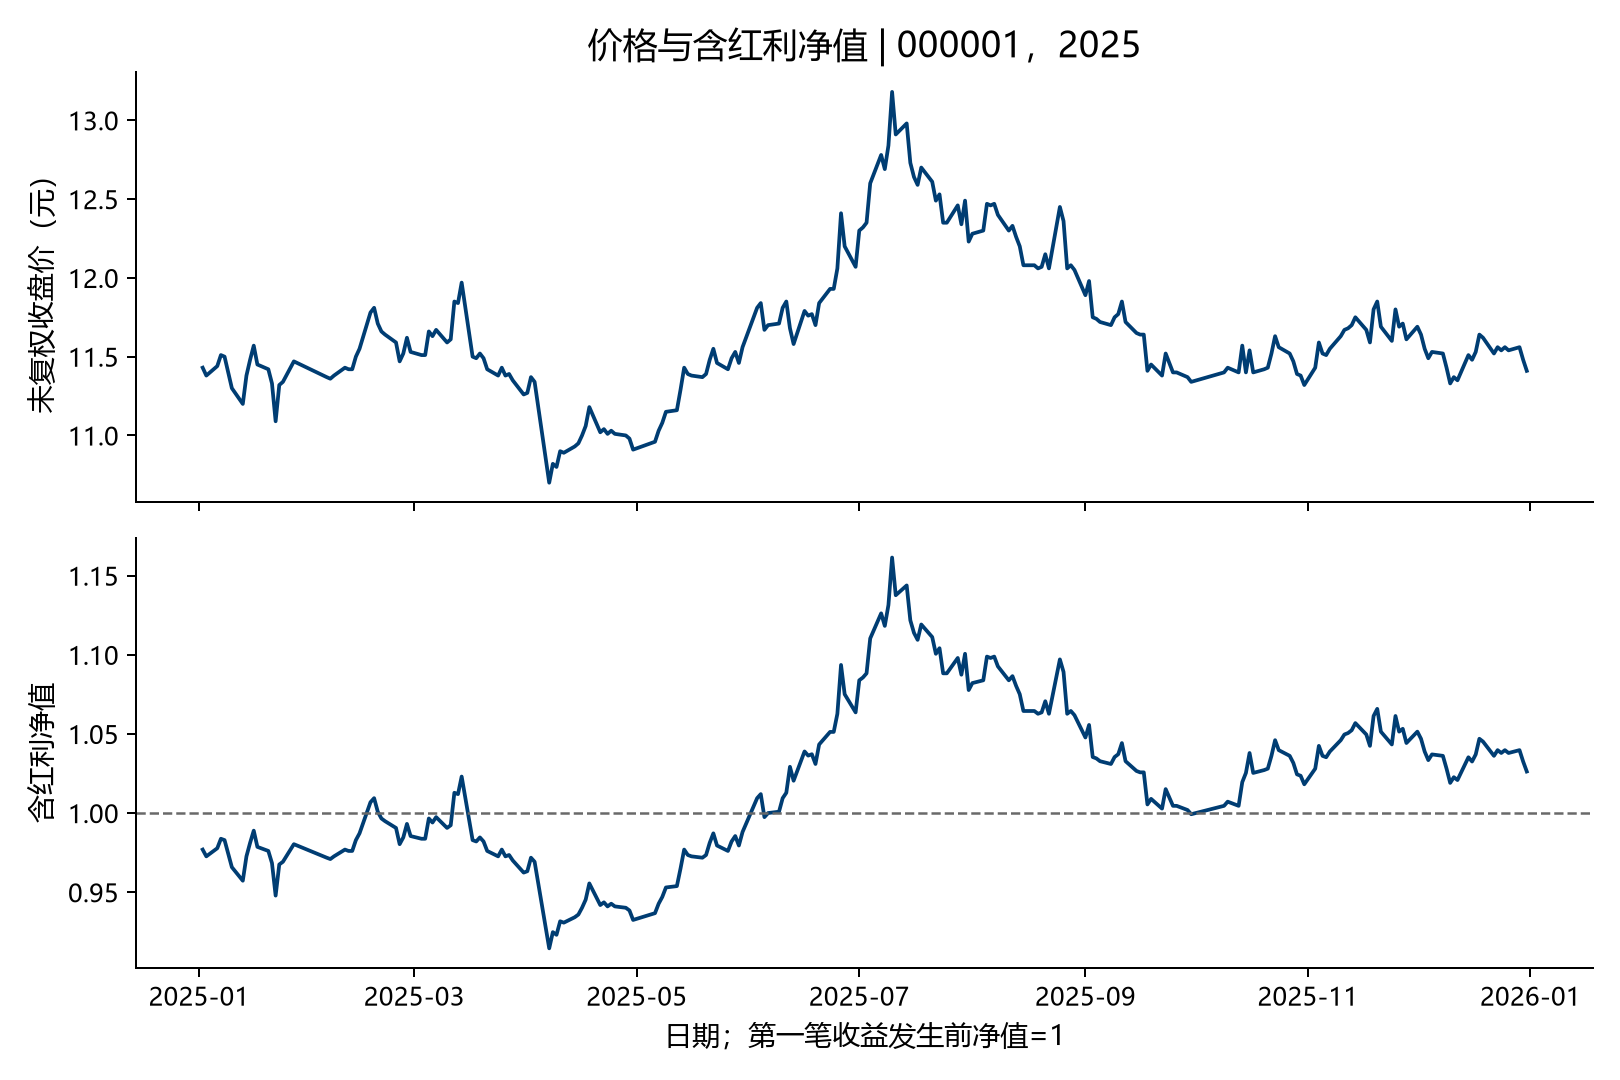
\includegraphics[height=6.15cm,width=.96\textwidth,keepaspectratio]{price_wealth.png}
  \nbref{4.1；证券代码000001，第一笔收益发生前净值=1}
\end{frame}

\begin{frame}[fragile]{对数收益率：方便跨期相加}
  \[
    g_t=\ln(1+r_t),\qquad
    \sum_{t=1}^{T}g_t=\ln\left[\prod_{t=1}^{T}(1+r_t)\right]
  \]
\begin{lstlisting}[numbers=none]
stock["log_return"] = np.log1p(stock["return"])
log_based = np.expm1(stock["log_return"].sum())
np.isclose(log_based, cumulative_return)
\end{lstlisting}
  \begin{itemize}
    \item \texttt{log1p(x)} 计算 $\ln(1+x)$；\texttt{expm1(x)} 计算 $e^x-1$。
    \item 收益率较小时，简单收益和对数收益接近，但并不相同。
    \item 当 $r\leq-1$ 时不能直接取对数，因此先检查输入。
    \item 对数收益可跨期相加；不能据此说不同资产的组合收益也直接等于对数收益的加权平均。
  \end{itemize}
  \nbref{4.1：两条计算路径结果核对}
\end{frame}

\begin{frame}[fragile]{波动率：收益率在均值附近有多分散？}
  \[
    s=\sqrt{\frac{1}{n-1}\sum_{t=1}^{n}(r_t-\bar r)^2},\qquad
    \sigma_{ann}\approx s\sqrt{252}
  \]
\begin{lstlisting}[numbers=none]
daily_vol = stock["return"].std(ddof=1)
annual_vol = daily_vol * np.sqrt(252)
vol20 = stock["return"].rolling(20).std() * np.sqrt(252)
\end{lstlisting}
  \begin{itemize}
    \item pandas 样本标准差默认采用分母 $n-1$。
    \item 252是年化约定，本章2025年样本实际有 \SampleDays{} 个日期。
    \item 平方根年化是近似：需要可比日频观测等假设，不是未来波动预测。
    \item 20观测滚动窗口不是20个自然日；开始的19条结果为空。
  \end{itemize}
  \nbref{4.2}
\end{frame}

\begin{frame}[fragile]{回撤：距离历史最高净值有多远？}
  \[
    DD_t=\frac{W_t}{\max(1,W_1,\ldots,W_t)}-1,\qquad
    MDD=\min_t DD_t
  \]
\begin{lstlisting}[numbers=none]
peak = stock["wealth"].cummax().clip(lower=1)
stock["drawdown"] = stock["wealth"] / peak - 1
max_drawdown = stock["drawdown"].min()
\end{lstlisting}
  \begin{itemize}
    \item 本章用负值报告回撤；越负代表距离峰值越远。
    \item 将初始投入1纳入峰值，避免忽略样本第一天就亏损的情况。
    \item 示例000001累计收益为 \TargetCum\%，但期间最大回撤为 \TargetMdd\%。
    \item 年末回报不能反映持有过程中的全部风险。
  \end{itemize}
  \nbref{4.2}
\end{frame}

\begin{frame}{滚动波动率与回撤展示风险的变化}
  \centering
  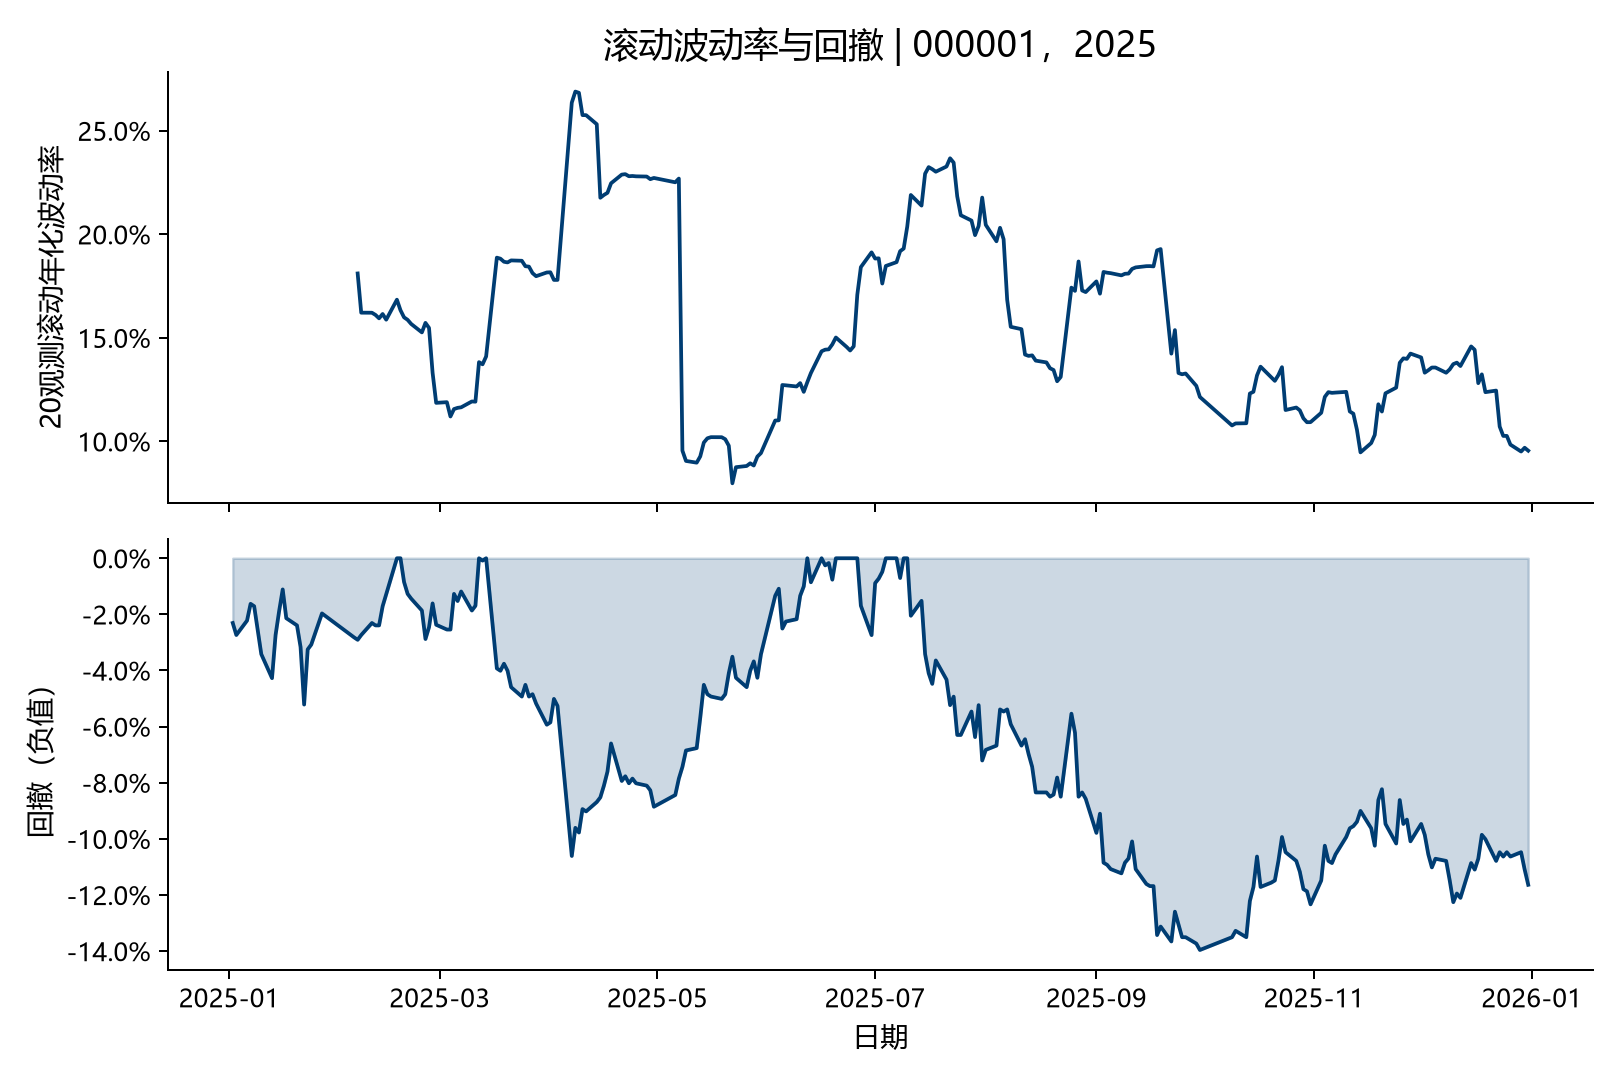
\includegraphics[height=6.1cm,width=.96\textwidth,keepaspectratio]{vol_drawdown.png}
  \nbref{4.2；000001全年近似年化波动率为 \TargetVol\%}
\end{frame}

\begin{frame}{成交量、成交额、市值与换手率}
  \begin{tabular}{p{0.25\textwidth}p{0.62\textwidth}}
    \toprule
    指标 & 经济含义与单位 \\
    \midrule
    成交量 & \texttt{Dnshrtrd}：一天成交多少股 \\[6pt]
    成交额 & \texttt{Dnvaltrd}：一天成交多少人民币元 \\[6pt]
    流通市值 & \texttt{Dsmvosd}：流通股数乘收盘价，\textbf{单位千元} \\[6pt]
    估算换手率 & 成交股数 / 由流通市值反推的流通股数 \\
    \bottomrule
  \end{tabular}
  \[
    S_t^{float}\approx\frac{\texttt{Dsmvosd}_t\times1000}{P_t},\qquad
    Turnover_t=\frac{Volume_t}{S_t^{float}}
  \]
  \begin{block}{单位不统一，结果会差1000倍}
    市值先从千元转为元。这里使用本包流通市值口径估算，不能称为官方自由流通换手率。
  \end{block}
  \nbref{第5节}
\end{frame}

\begin{frame}[fragile]{用 pandas 制作几个基本指标}
\begin{lstlisting}[numbers=none]
df["amount_100m"] = df["Dnvaltrd"] / 1e8
df["float_mv_100m"] = df["Dsmvosd"] * 1000 / 1e8
shares = df["Dsmvosd"] * 1000 / df["Clsprc"]
df["turnover"] = df["Dnshrtrd"] / shares.where(shares > 0)
df["intraday_range"] = (
    (df["Hiprc"] - df["Loprc"]) / df["PreClosePrice"]
)
\end{lstlisting}
  \begin{itemize}
    \item 成交额、市值统一到亿元，便于表格和图形展示。
    \item 日内高低价范围是日频摘要，不能还原盘中路径。
    \item 比率分母为0或缺失时，先处理口径；不要把不可计算的比率填成0。
    \item Notebook 对昨收价格也只在大于0时计算范围指标。
  \end{itemize}
  \nbref{第5节}
\end{frame}

\section{描述性统计与可视化}
\begin{frame}{平均值之前，先问“对谁求平均”？}
  \begin{tabular}{p{0.27\textwidth}p{0.6\textwidth}}
    \toprule
    观察单位 & 回答的问题 \\
    \midrule
    单只股票的日期 & 这只股票在一段时间内如何表现？ \\[10pt]
    同一天的各股票 & 当天样本股票的横截面分布如何？ \\[10pt]
    全部股票日混合 & 本样本所有可用股票日的总体分布如何？ \\[10pt]
    每只股票的年度汇总 & 不同股票的区间回报和风险如何比较？ \\
    \bottomrule
  \end{tabular}
  \begin{block}{本章的全样本均值}
    每条股票日等权；观测较多的股票贡献更多行。\par
    它不是官方指数收益率，也不是一个已经定义好的投资组合年收益率。
  \end{block}
  \nbref{第6、7节}
\end{frame}

\begin{frame}{描述性统计：中心、离散程度与尾部}
  \centering
  \begin{tabular}{lrl}
    \toprule
    \SampleYear{} 年股票日统计 & 数值 & 含义 \\
    \midrule
    均值 & \ReturnMean\% & 中心，会受极值影响 \\
    中位数 & \ReturnMedian\% & 一半观测在其上下 \\
    日标准差 & \ReturnStd\% & 混合分布的离散程度 \\
    1\%分位数 & \ReturnLow\% & 左尾位置 \\
    99\%分位数 & \ReturnHigh\% & 右尾位置 \\
    最小值 & \ReturnMin\% & 样本最小单日回报 \\
    最大值 & \ReturnMax\% & 样本最大单日回报 \\
    \bottomrule
  \end{tabular}
  \begin{block}{为什么均值和中位数差别值得关注？}
    本样本含极大的正收益记录。平均值、标准差与高阶矩可能被少数事件显著影响，应配合分位数和业务核验。
  \end{block}
  \nbref{第6节；所有数值以含红利收益率计算}
\end{frame}

\begin{frame}{分布图：全样本与局部放大同时看}
  \centering
  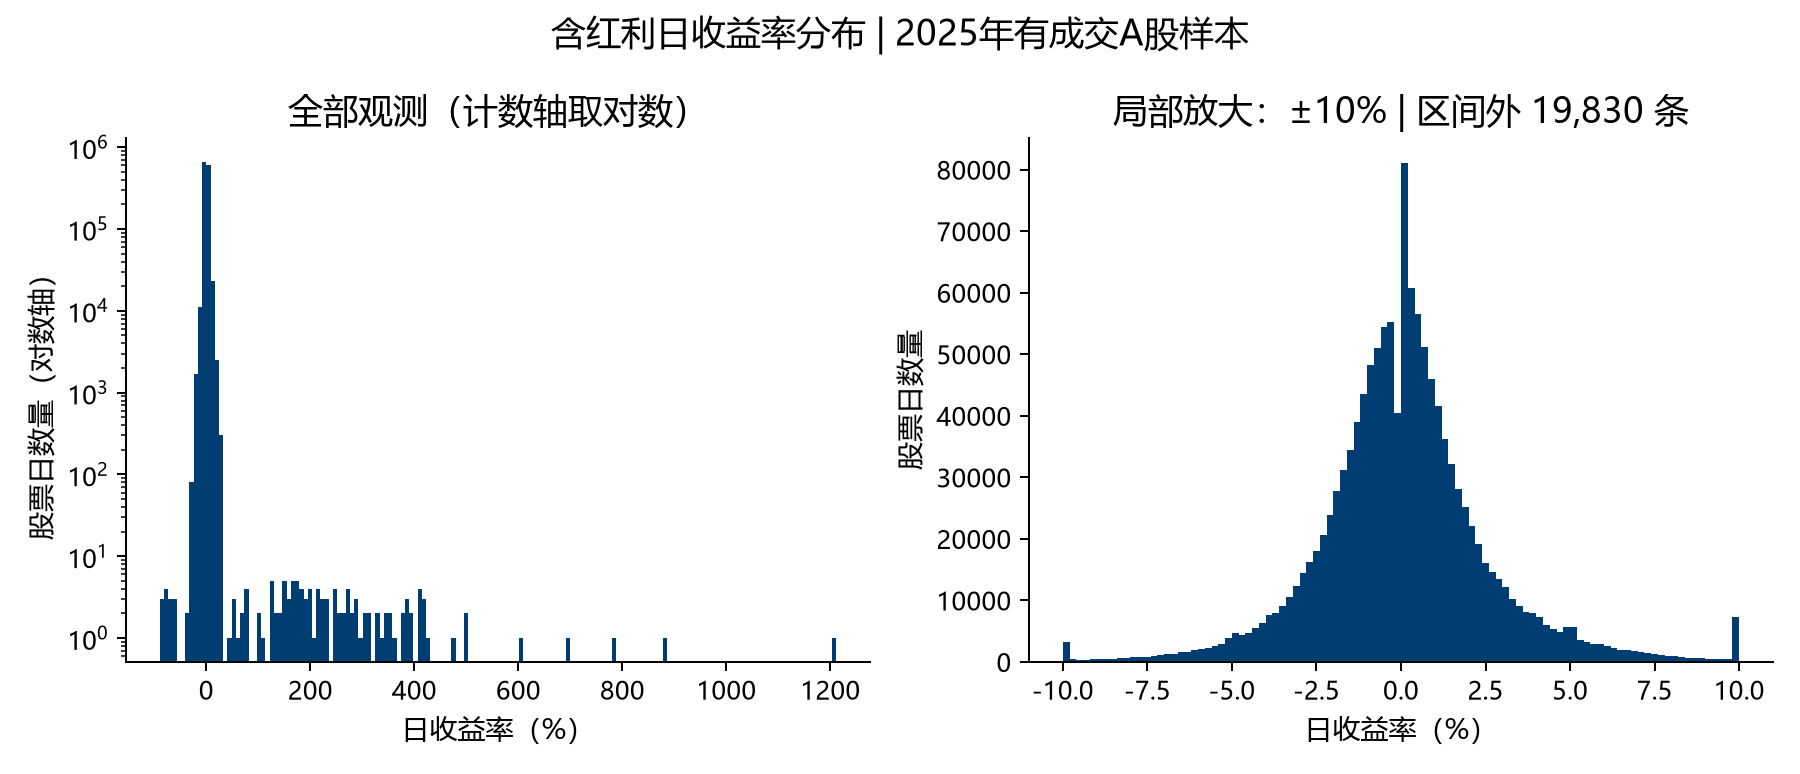
\includegraphics[width=\textwidth,height=5.2cm,keepaspectratio]{return_distribution.png}
  \begin{itemize}
    \item 左图保留全部极值并使用对数计数轴；右图仅放大正负10\%区间。
    \item 右图没有改变统计样本，区间外数量已标注。
    \item 本样本偏度为 \ReturnSkew{}，超额峰度为 \ReturnKurt{}；高阶矩受极端事件影响很大。
  \end{itemize}
  \nbref{6.1；pandas的 \texttt{kurt()} 是超额峰度，正态分布为0}
\end{frame}

\begin{frame}{极值核验：大涨大跌不一定是数据错误}
  \begin{block}{正向极值：920091，2025-11-21}
    本包含红利日回报约 \textbf{+1211.11\%}。北交所披露确认该日为上市首日，发行价9元。\par
    该收益的起点是发行价，不能理解为首日开盘买入就能获得。
  \end{block}
  \begin{block}{负向极值：000622，2025-06-25}
    本包日回报约 \textbf{-89.33\%}。公司披露确认该日进入退市整理期，首日不设价格涨跌幅限制。
  \end{block}
  \begin{itemize}
    \item 核对了这两条记录的事件背景和表内价格公式；不是全部极值已核验。
    \item 不机械截断到正负10\%；\texttt{LimitStatus} 缺失也不能当“未涨跌停”。
  \end{itemize}
  \sourcehint{https://www.bse.cn/issue_report_meeting/200027211.html}{北交所：大鹏工业上市报道}
  \sourcehint{https://disc.static.szse.cn/disc/disk03/finalpage/2025-06-19/ac36f03f-1bba-480d-9012-df4c030c22cb.PDF}{公司退市公告，深交所披露}
\end{frame}

\begin{frame}{不同板块的分布可以怎样比较？}
  \centering
  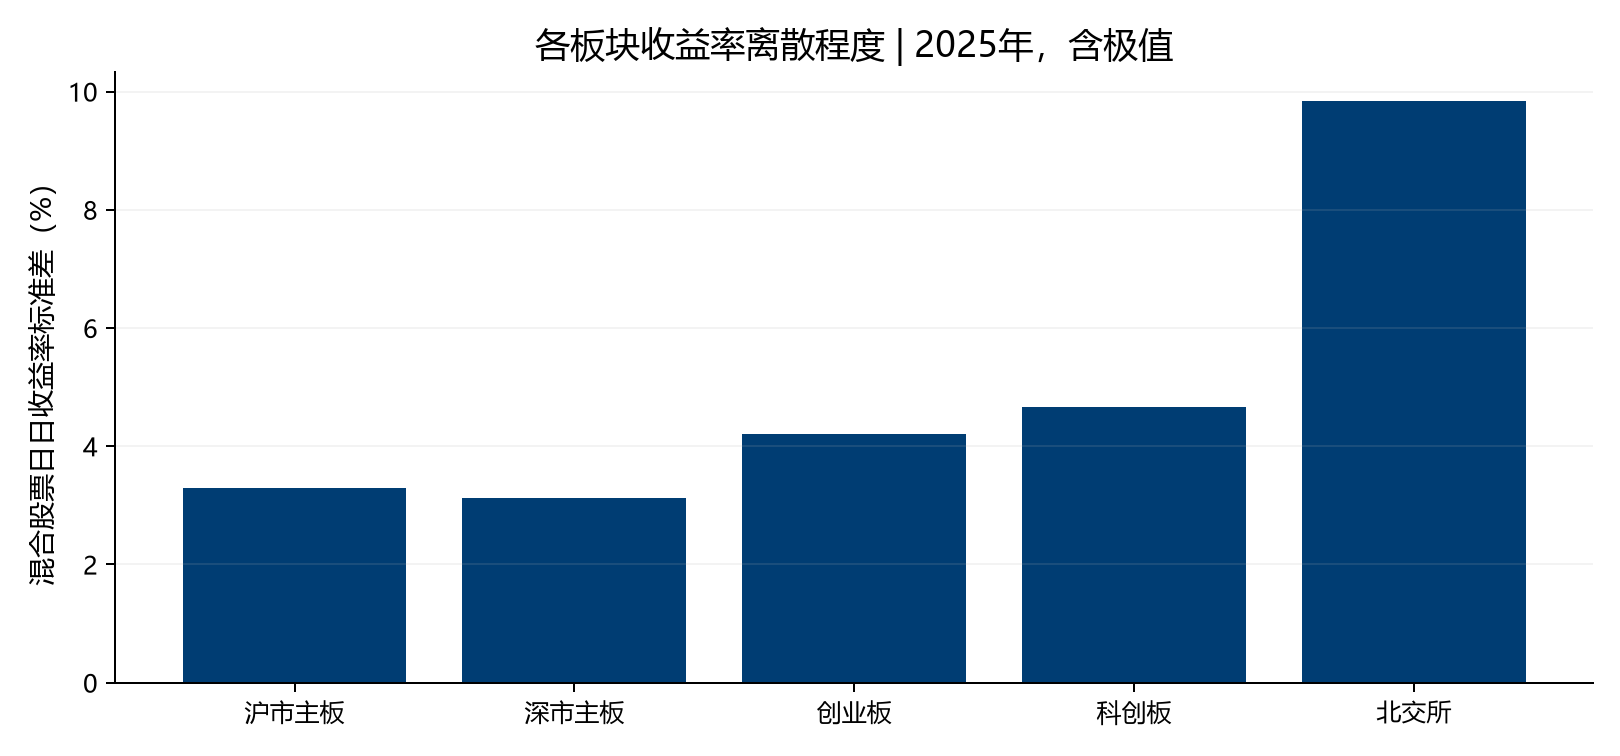
\includegraphics[width=.97\textwidth,height=5.1cm,keepaspectratio]{board_dispersion.png}
  \begin{itemize}
    \item 此图是板块内\textbf{全部股票日混合}标准差，不是“典型股票”的年化波动率。
    \item 包含新股与极值；板块差异也可能来自行业、规模和上市时间。
    \item 观察到差异不等于板块本身造成收益或风险差异。
  \end{itemize}
  \nbref{6.2：\texttt{groupby().agg()}}
\end{frame}

\begin{frame}{跨股票比较：先限制有效观测数量}
  \centering
  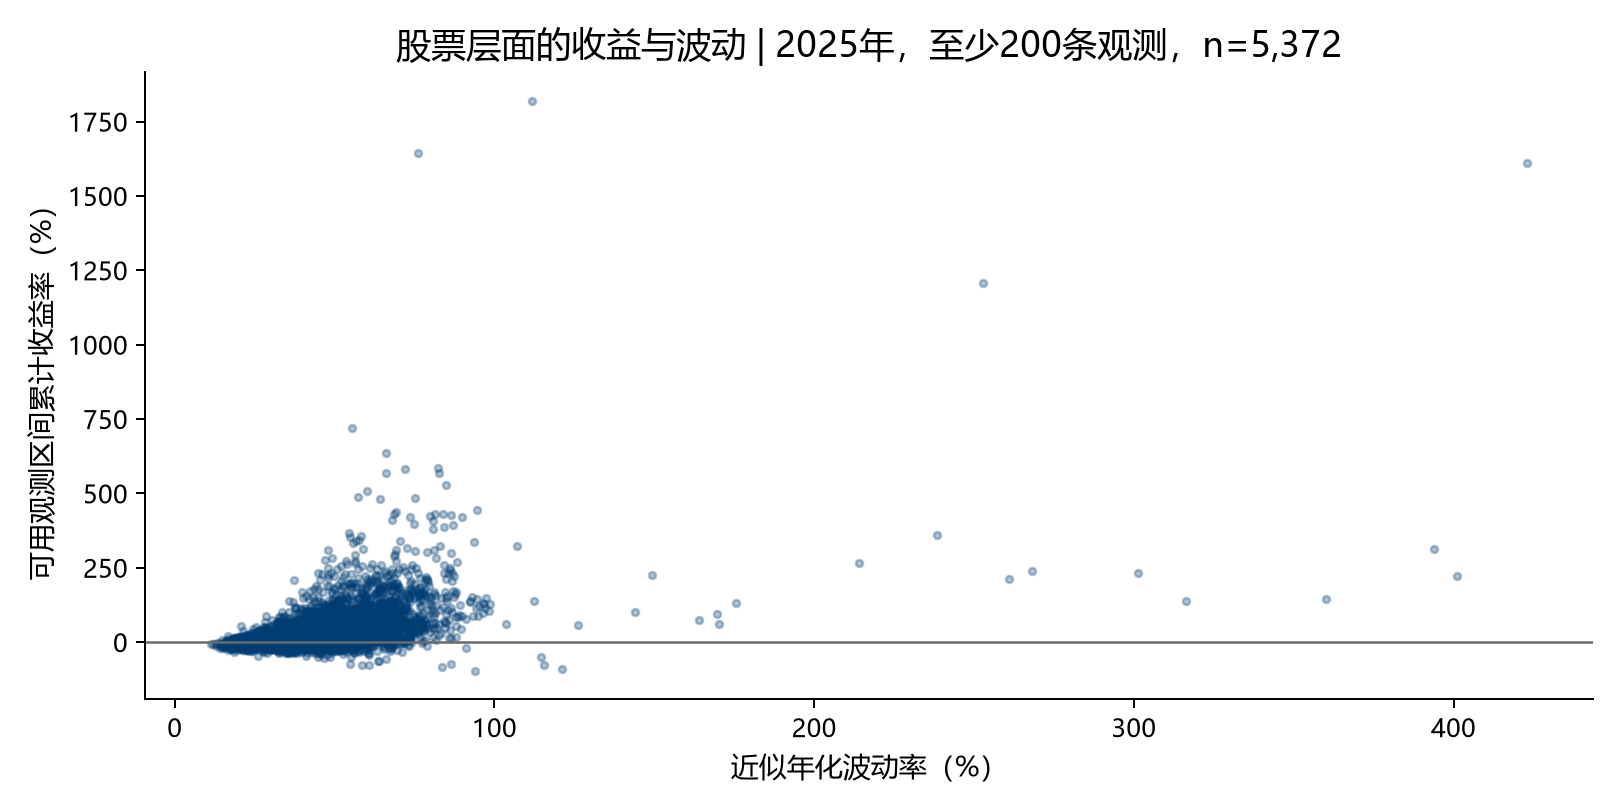
\includegraphics[width=.98\textwidth,height=5.1cm,keepaspectratio]{risk_return.png}
  \begin{itemize}
    \item 每点是一个代码，至少200条观测；仍可能覆盖不同起止日期。
    \item 横轴为近似年化波动率，纵轴为代码的可用观测区间累计回报。
    \item 未做跨代码衔接、成本处理或策略回测，不能直接据此选股。
  \end{itemize}
  \nbref{第7节：逐代码汇总}
\end{frame}

\begin{frame}{相关性：先对齐共同有效日期}
  \centering
  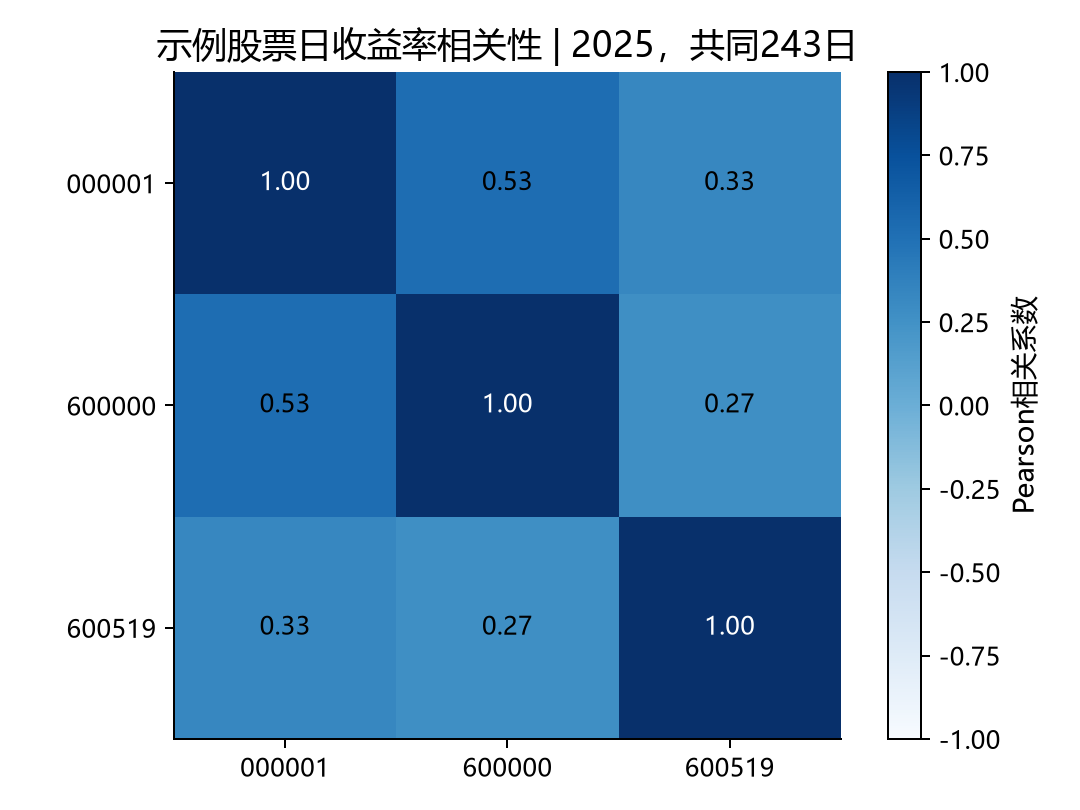
\includegraphics[height=5.35cm,width=.9\textwidth,keepaspectratio]{correlation.png}
  \begin{itemize}
    \item 三个示例代码使用共同有效日期；不把缺失收益补成0。
    \item 相关性描述历史共同变化，不代表因果或未来稳定关系。
  \end{itemize}
  \nbref{第7节：\texttt{pivot → dropna → corr}}
\end{frame}

\section{复现与解释结果}
\begin{frame}{从原始数据到课件：一条可重复的路径}
  \begin{enumerate}
    \item \textbf{原始ZIP}：Notebook列出包内文件，并解压到本地目录。
    \item \textbf{读取CSV}：先试读，再逐块读取7个文件、选择年份、合并和检查。
    \item \textbf{开展分析}：接着展示A股样本筛选、指标计算、图表和核验。
    \item \textbf{汇总结果}：保存筛选表、板块表、统计表、相关系数及7张图。
    \item \textbf{课件}：引用相同图表与自动生成的统计宏。
  \end{enumerate}
  \begin{block}{本章文件位置}
    \texttt{data/raw/}\quad Notebook解压得到的原始文件\par
    \texttt{notebooks/11\_股票日频收益率分析.ipynb}\quad 从ZIP开始的完整流程\par
    \texttt{outputs/}\quad 汇总结果\par
    \texttt{latex/chapter11.tex}\quad 课件源码
  \end{block}
  更换分析参数后，需要重新执行 Notebook，并检查课件中的日期、案例与口径说明。
\end{frame}

\begin{frame}{本章应掌握的判断能力}
  \begin{itemize}
    \item 看数据先确认观察单位、时间范围、证券范围和字段单位。
    \item 用合适的收益口径；累计收益相乘，对数收益跨期相加。
    \item 波动率、回撤与换手率描述不同维度，不应互相替代。
    \item 统计必须说明分母；用中位数、分位数和全分布辅助均值。
    \item 极值先查事件，缺失先查定义；保留数据处理的可追溯路径。
  \end{itemize}
  \begin{block}{继续思考}
    如果更换年份、只保留正常状态、改变最低观测数，结论是否改变？\par
    若要分析行业差异或投资组合，还需要补充哪些数据和假设？
  \end{block}
  \textbf{能生成统计表只是开始；能说明这些数代表什么，才是分析。}
\end{frame}

\begin{frame}{数据与资料来源}
  \small
  \begin{itemize}
    \item CSMAR 本地授权包：\texttt{TRDNEW\_Dalyr}，7个CSV；字段口径以包内说明为准。
    \item \href{https://star.sse.com.cn/assortment/stock/list/share/}{上海证券交易所：股票分类}。
    \item \href{https://www.szse.cn/aboutus/trends/news/t20210406_585442.html}{深圳证券交易所：2021年4月6日两板合并}。
    \item \href{https://www.bse.cn/company/introduce.html}{北京证券交易所：本所简介}。
    \item \href{https://www.bse.cn/issue_report_meeting/200027211.html}{北交所：920091于2025年11月21日上市，发行价9元}。
    \item \href{https://disc.static.szse.cn/disc/disk03/finalpage/2025-06-19/ac36f03f-1bba-480d-9012-df4c030c22cb.PDF}{000622公司退市公告：2025年6月25日进入退市整理期}。
  \end{itemize}
  \vspace{0.3cm}
  官网核对日期：2026-09-09。\par
  市场结构背景、原包字段定义、计算出的样本统计分别标识，不将样本统计冒充官方市场全貌。
\end{frame}
\end{document}
